\section{Forces in Equilibrium}

%Moments / Turning Forces

\subsection{Door Tug-o-War}
\begin{itemize}
\item{Preparation time: none}
\item{Materials: a strong door}
\item{Procedure: Get 2 students. One is going to push against the door near the hinge; one will push the other way near the other side (handle) of the door. The one pushing near the edge of the door will find it easy to push the door her way.}
\item{Theory: The student that pushes farther from the axis of rotation can exert less force, but still produce a greater torque, or moment of force, than the one pushing close to the hinge, because.}
\end{itemize}


%Principle of Moments

%\subsection{Twenty Shillings of Equilibrium}
%\begin{itemize}
%\item{Preparation Time: none}
%\item{Materials: Meter rule, handful of 20/= coins}
%\item{Procedure: Balance the meter rule on your forefinger at the 50 cm mark. Discuss the idea of equilibrium and equal moments. Place one coin at the 1 m mark and watch the rule rotate and the coin fall, demonstrating a lack of equilibrium. Now replace the coin and add another coin to the 0 m mark. The meter rule should stay steady. For more numerical fun, add two coins at the 25 cm mark, four coins at the 12.5 cm mark, and even eight coins at 6.25 cm if you dare! Have students calculate the necessary lengths or masses (number of coins – we do not need actual units here since the masses are equal) while you perform the daring feats in front.}
%\item{Theory: The moment of a force is equal to the force times the distance from the pivot. The pivot is your finger and the forces are all at even intervals. If the total moment in the clockwise direction is equal to the moment in the anticlockwise direction, you have equilibrium. You can add or remove coins, change distances, etc. while still keeping the moments equal.}
%\end{itemize}


\subsection{Verification of the Principle of Moments}

\subsubsection*{Learning Objectives}
\begin{itemize}
\item{To determine the moment of forces of a uniform wooden bar}
\end{itemize}

\subsubsection*{Background Information}
The body will be in equilibrium when the clockwise moments equal the anticlockwise moments. The turning forces depend on the product of the distance from the pivot to the point of application of the force and the magnitude of the perpendicular forces acting on the mass.  

\subsubsection*{Materials}
Metre rule, three dry cells or any two objects of equal weight, thread, triangular wooden block or any object that will create a pivot point.  

\begin{figure}[h]
\begin{center}
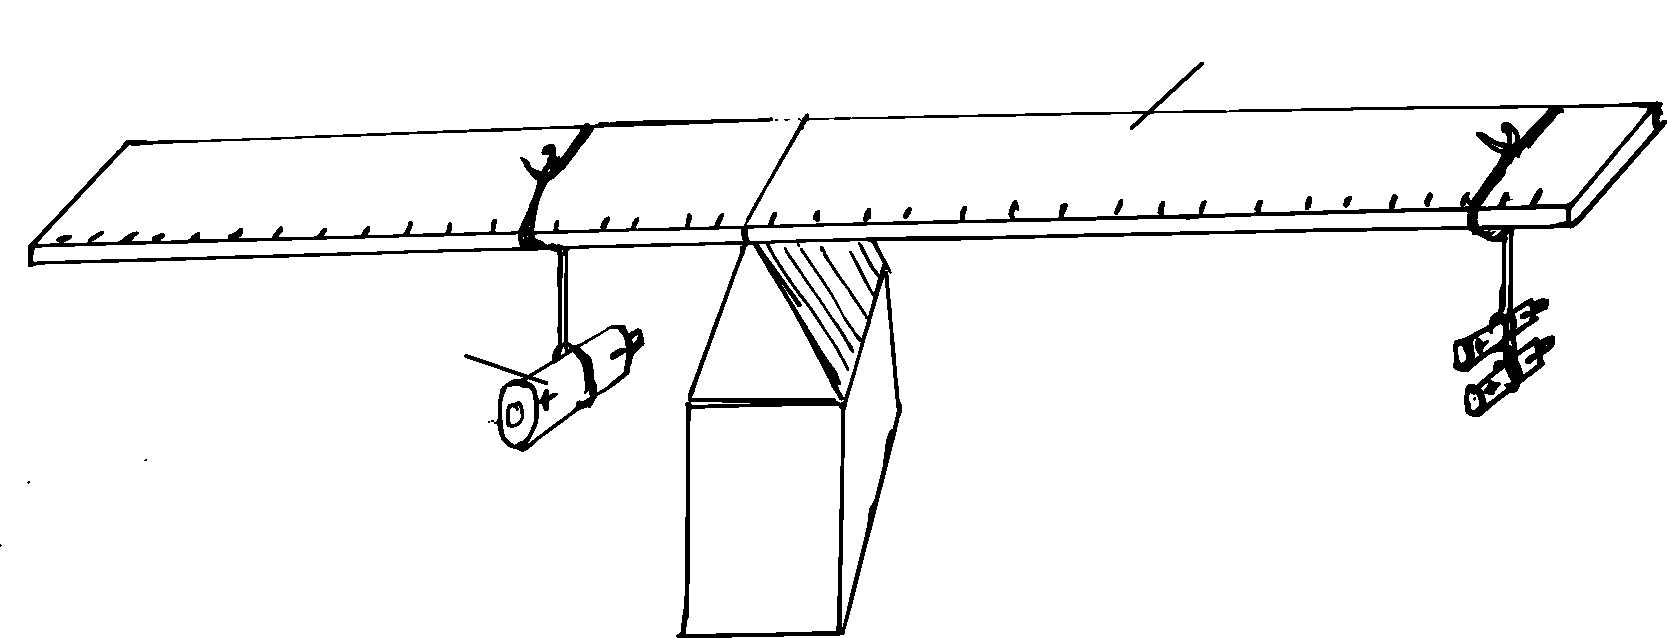
\includegraphics{./img/equilibrium-moment.png}
\caption{Equilibrium of Moments}
\label{fig:equilibrium-moment}
\end{center}
\end{figure}

\subsubsection*{Activity Procedure}
\begin{enumerate}
\item{Balance the metre rule on the pivot point so that it remains horizontal.} 
\item{Place two equal weights 20 cm from the pivot on the right and left sides of the pivot so that the ruler remains balanced.} 
\item{Now move the right weight 5 cm further away from the pivot point and observe what happens.} 
\item{Return that weight to the 20 cm mark and the system back to equilibrium. Now move the same weight 5 cm closer to the pivot point and observe what happens.} 
\item{Now balance the metre rule itself on the pivot and place one weight at the 20~cm on the left side of the pivot and the two other weights at the 10~cm mark on the opposite side of the pivot. The metre rule should remain balanced.} 
\end{enumerate}

\subsubsection*{Results and Conclusions}
When the system is in equilibrium the product of the distance to the pivot point and the weight on opposite sides of the pivot are equal.  

\subsubsection*{Clean Up Procedure}
Put the instruments back in their respective places.

\subsubsection*{Discussion Question}
Explain the relation between the masses and distance from the pivot when the metre rule is at equilibrium.

\subsubsection*{Notes}
The wooden bar or metre rule should be uniform in order to simplify this experiment.
Many objects and tools operate by the principle of moments.  For a turning force to be more effective, the distance of the force from the pivot should be large.  A force close to the pivot will have a smaller effect.  This explains why the handle of a door is far from the hinge, or why a bottle opener has a long handle.



%Centre of Gravity

\subsection{Centre of Gravity}

\subsubsection*{Learning Objectives}
\begin{itemize}
\item{To determine the centre of gravity of uniform wooden rod} 
\end{itemize}

\subsubsection*{Background Information}
The weight of object is concentrate at single point. This point is called the centre of gravity. For a uniform rod, the centre of gravity is normally at the centre of the rod.  Finding the center of gravity is something used often in daily life -- especially when balancing a bucket or large stick on the head.

\subsubsection*{Materials}
Uniform wooden rod about 1 m long, triangular blocks, ruler, wooden block

\subsubsection*{Activity Procedure}
\begin{enumerate}
\item{Place the wooden block on the table.} 
\item{Place the triangular block on the table so that the sharp edge is pointing upward.} 
\item{Slowly place the wooden rod on top of sharp edge of the triangle block and move it until it balances horizontally.} 
\item{Mark this balancing point on the wooden rod and measure its distance from both ends.} 
\end{enumerate}

\begin{figure}
\begin{center}
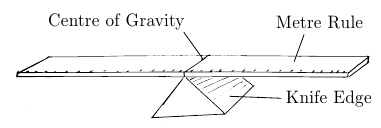
\includegraphics{./img/centre-of-gravity.png}
\caption{Finding the Centre of Gravity}
\label{fig:center-of-gravity}
\end{center}
\end{figure}

\subsubsection*{Results and Conclusions}
The wooden bar balances near the middle. The balance point is known as the centre of gravity.  

\subsubsection*{Clean Up Procedure}
Collect all materials and return them to their proper places.

\subsubsection*{Discussion Questions}
\begin{enumerate}
\item{Was the centre of gravity at the centre of the wooden rod? How do you know?}
\item{Discuss another method to locate the centre of gravity of a uniform rod.} 
\end{enumerate}


%Types of Equilibrium